\documentclass[tikz,border=2]{standalone}
%% \usepackage{amsfonts}
\usepackage{lmodern} % enhanced version of computer modern
\usepackage[T1]{fontenc} % for hyphenated characters
\usepackage{amssymb}
\usepackage{amsmath}
\usepackage{amsthm}
%
\usetikzlibrary{decorations.pathreplacing,shadows,arrows,shapes,positioning,calc,backgrounds,fit}
\newcommand{\mA}{\mathcal{A}}
\newcommand{\mB}{\mathcal{B}}
\newcommand{\mC}{\mathcal{C}}
\newcommand{\mI}{\mathcal{I}}
\newcommand{\mN}{\mathcal{N}}
\newcommand{\mP}{\mathcal{P}}
\newcommand{\mR}{\mathcal{R}}
\newcommand{\mS}{\mathcal{S}}
\newcommand{\mY}{\mathcal{Y}}
% Define the layers to draw the diagram
%
\begin{document}
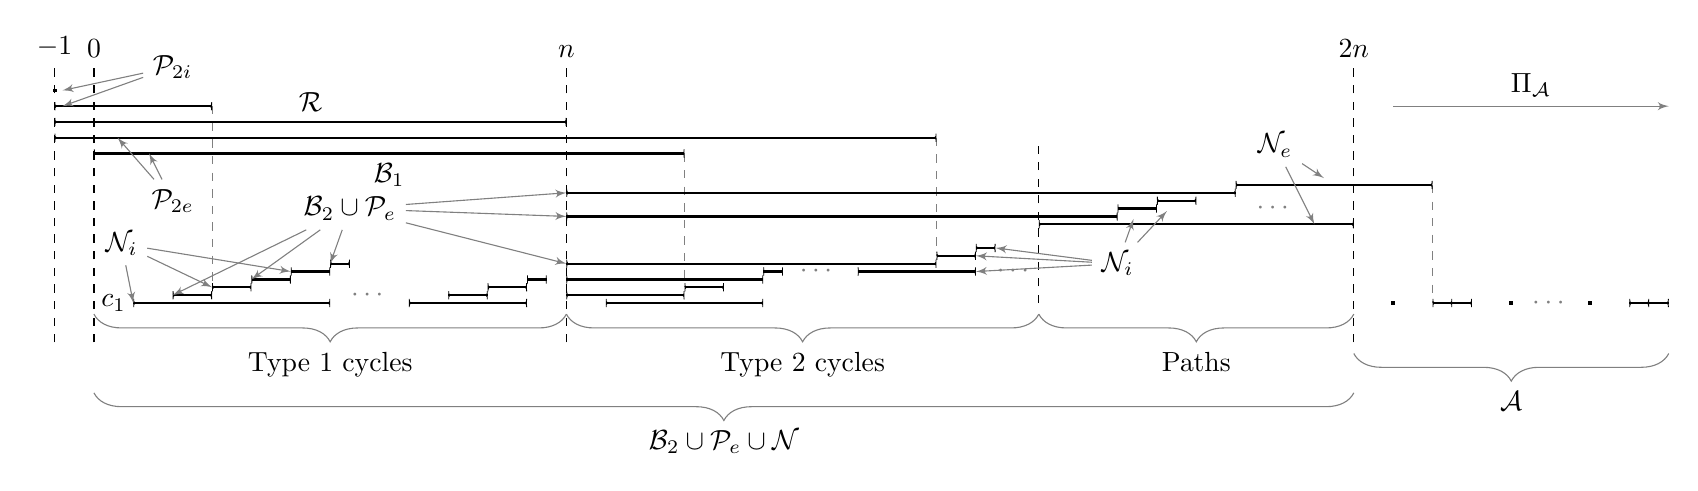
\begin{tikzpicture}
[node distance=1cm,
interval/.style={thick,>=serif cm,rounded corners=1.24pt},
uint/.style={shape=rectangle,draw=black,inner sep=.5pt,fill},
dedge/.style={gray,>=latex', shorten >=.0pt, shorten <=.0pt},
myedge/.style={thick}]
%%
% boundaries
%%
\draw[dashed] (-.5,-1.5) -- (-.5,2) node[above] (m1) {$-1$};
\draw[dashed] (0,-1.5) -- (0,2) node[above] (0) {$0$};
\draw[dashed] (6,-1.5) -- (6,2) node[above] (n) {$n$};
\draw[dashed] (12,-1) -- (12,1) node[above] (Type2) {};
\draw[dashed] (16,-1.5) -- (16,2) node[above] (2n) {$2n$};
%%
% A
\path (16,-1) 
++(.5,0) node[uint] {}
++(.5,0) edge[interval,<->] +(.25,0)
++(.5,0) edge[interval,<-] +(-.25,0)
++(.5,0) node[uint] {}
++(.5,0) node[gray] {$\cdots$}
++(.5,0) node[uint] {}
++(.5,0) edge[interval,<->] +(.25,0)
++(.5,0) edge[interval,<-] +(-.25,0);
\draw [gray,decorate,decoration={brace,amplitude=10pt,mirror,raise=4pt},yshift=0pt]
(16,-1.5) -- (20,-1.5) node [midway,below,yshift=-.5cm,black] {$\mA$};
\draw [dedge,->] (16.5,1.5) -- (20,1.5) node [midway,above,black]
{${\Pi_{\mA}}$};
%%
% B2PeN
%%
\draw [gray,decorate,decoration={brace,amplitude=10pt,mirror,raise=4pt},yshift=0pt]
(0,-2) -- (16,-2) node [midway,below,yshift=-.5cm,black] {$\mB_2\cup\mP_e\cup\mN$};
\draw [gray,decorate,decoration={brace,amplitude=10pt,mirror,raise=4pt},yshift=0pt]
(0,-1) -- (6,-1) node [midway,below,yshift=-.5cm,black] {Type 1 cycles};
\draw [gray,decorate,decoration={brace,amplitude=10pt,mirror,raise=4pt},yshift=0pt]
(6,-1) -- (12,-1) node [midway,below,yshift=-.5cm,black] {Type 2 cycles};
\draw [gray,decorate,decoration={brace,amplitude=10pt,mirror,raise=4pt},yshift=0pt]
(12,-1) -- (16,-1) node [midway,below,yshift=-.5cm,black] {Paths};
%%
% Type 1
%%
\path (0,-1)
++(.5,0) edge[interval,<->] +(2.5,0)
++(.5,.1) edge[interval,<->] +(.5,0)
++(.5,.1) edge[interval,<->] +(.5,0)
++(.5,.1) edge[interval,<->] +(.5,0)
++(.5,.1) edge[interval,<->] +(.5,0)
++(.5,.1) edge[interval,<->] +(.25,0)
++(.5,-.4) node[gray] {$\cdots$}
++(.5,-.1) edge[interval,<->] +(1.5,0)
++(.5,.1) edge[interval,<->] +(.5,0)
++(.5,.1) edge[interval,<->] +(.5,0)
++(.5,.1) edge[interval,<->] +(.25,0);
%%
\node at (0.25,-1) {$c_1$};
%%
\node at (0.35,-.25) (Ni) {$\mN_i$};
\path 
(Ni) edge[dedge,->] (.5,-1)
(Ni) edge[dedge,->] (1.5,-.8)
(Ni) edge[dedge,->] (2.5,-.6);
%%
\node at (3.25,0.2) (B2Pe) {$\mB_2\cup\mP_e$};
\path 
(B2Pe) edge[dedge,->] (1,-.9)
(B2Pe) edge[dedge,->] (2,-.7)
(B2Pe) edge[dedge,->] (3,-.5)
(B2Pe) edge[dedge,->] (6,.4)
(B2Pe) edge[dedge,->] (6,0.1)
(B2Pe) edge[dedge,->] (6,-.5);
%%
% Type 2
%%
\path (6,-1)
++(.5,0) edge[interval,<->] +(2,0)
+(-.5,.1) edge[interval,<->] +(1,.1)
++(1,.2) edge[interval,<->] +(.5,0)
+(-1.5,.1) edge[interval,<->] +(1,.1)
++(1,.2) edge[interval,<->] +(.25,0)
++(.7,0) node[gray] {$\cdots$}
++(.5,0) edge[interval,<->] +(1.5,0)
+(-3.7,.1) edge[interval,<->] +(1,.1)
++(1,.2) edge[interval,<->] +(.5,0)
++(.5,.1) edge[interval,<->] +(.25,0)
++(.5,-.3) node[gray] {$\cdots$};
%%
% Paths
%%
\path (12,0)
(12,0) edge[interval,<->] node (ne1){} (16,0)
(6,.1) edge[interval,<->] (13,.1)
(13,.2) edge[interval,<->]node (ni1){}  (13.5,.2)
(13.5,.3) edge[interval,<->] node (ni2){} (14,.3)
(6,.4) edge[interval,<->] (14.5,.4)
(14.5,.5) edge[interval,<->] node (ne2){} (17,.5)
(15,.2) node[gray] {$\cdots$};
%%
\node at (13,-.5) (Ni) {$\mN_i$};
\path 
(Ni) edge[dedge,->] (11.2,-.6)
(Ni) edge[dedge,->] (11.2,-.4)
(Ni) edge[dedge,->] (11.45,-.3)
(Ni) edge[dedge,->] (ni1)
(Ni) edge[dedge,->] (ni2);
%%
\node at (15,1) (Ne) {$\mN_e$};
\path 
(Ne) edge[dedge,->] ([xshift=1.5cm] ne1)
(Ne) edge[dedge,->] (ne2);
%%
% B1, P2e, R and P2i
%%
\path 
(0,.9) edge[interval,<->] node [midway,below] {$\mB_1$} (7.5,.9)
(-.5,1.1) edge[interval,<->] (10.7,1.1)
(-.5,1.3) edge[interval,<->] node [midway,above] {$\mR$} (6,1.3)
(-.5,1.5) edge[interval,<->] (1.5,1.5) 
(-.5,1.7) node[uint] (p2i) {};
%
\node at (1,2) (P2i) {$\mP_{2i}$};
\path 
(P2i) edge[dedge,->] (-.4,1.5)
(P2i) edge[dedge,->] (-.4,1.7);
%
\node at (1,0.3) (P2e) {$\mP_{2e}$};
\path 
(P2e) edge[dedge,->] (.7,.9)
(P2e) edge[dedge,->] (.3,1.1);
%
\begin{pgfonlayer}{background}
\path
(7.5,.9) edge[dashed,gray] (7.5,-.8)
(10.7,1.1) edge[dashed,gray] (10.7,-.4)
(1.5,1.5) edge[dashed,gray] (1.5,-.8)
(17,.5) edge[dashed,gray] (17,-1);
\end{pgfonlayer}
\end{tikzpicture}
{}
\end{document}
